\begin{enumerate}

	\item The point which was misclassified as -1 in the $t$-th iteration will have the maximum weight in the next iteration as shown in Figure \ref{fig:problem_3_a}.
	
		\begin{figure*}
			\centering
			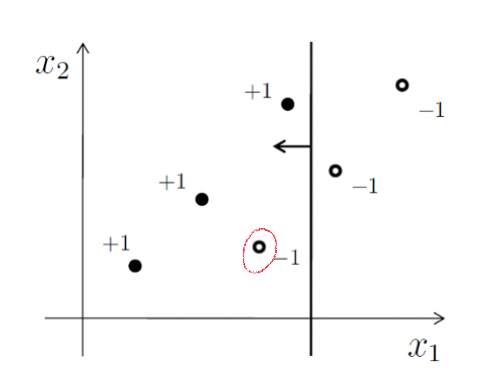
\includegraphics[width=0.5\textwidth]{images/problem_3_a.png}
			\caption{Point -1 (in red circle) is misclassified}
			\label{fig:problem_3_a}	
		\end{figure*}
		
	\item We know that the point misclassified in the previous iteration will have the highest probability of being selected in the next iteration. Assuming that the misclassified point was selected the model would try to reduce the error for that point and a possible stump would look like something shown in Figure \ref{fig:problem_3_b}. This also makes sense since now it is misclassifying only one point instead of two, in the previous iteration.
		
		\begin{figure*}[!ht]
			\centering
			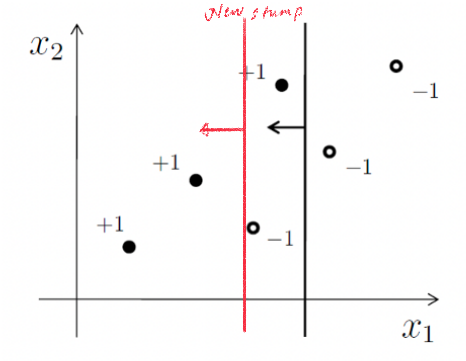
\includegraphics[width=0.5\textwidth]{images/problem_3_b.png}
			\caption{New stump (red line) for the next the boosting iteration}
			\label{fig:problem_3_b}	
		\end{figure*}
		
	\item Yes. As seen in the Figure \ref{fig:problem_3_b}, the second stump misclassifies one data point of class +1, whereas the first stump misclassified two data points (+1, -1). Thus, the relative weight $\alpha_{2}$ would be higher. $$\alpha_{2} > \alpha_{1}$$
        
\end{enumerate}
